\item

Wir berechnen zuerst Kandidaten für die Extrempunkte. Die Ableitungen lauten:

$f_x(x,y) = 4(y^2+10y)+9x^2$

$f_y(x,y) = 4(x-2)(2y+10)$

Aus $f_y = 0$ folgt $x=2 \lor y=-5$.

\begin{enumerate}
\item $x=2$

Wir setzen  $x=2$ in $f_x(x,y) = 0$ ein:

$f_x(2,y) = 0 = 4y^2+40y+36$

$\implies y = -5 \pm \sqrt{25-9}$

$\implies y = -9 \lor y = -1$

\item $y=-5$

$f_x(x,-5) = 0 = 4 \cdot (25-50)+9x^2 = -100+9x^2$

$\implies x^2 = \frac{100}{9}$

$\implies x=-\frac{10}{3} \lor x=\frac{10}{3}$

\end{enumerate}

Wir erhalten also die 4 möglichen Stellen $(2|-1), (2|-9), (\frac{10}{3}|-5)$ und $(-\frac{10}{3}|-5)$.

Zum Überprüfen, ob es sich um Minima, Maxima oder Sattelpunkte handelt, benötigen wir noch die 2. Ableitungen:

$f_{xy}(x,y) = 8(y+5)$

$f_{xx}(x,y) = 18x$

$f_{yy}(x,y) = 8(x-2)$

Wir erhalten damit für die 4 Stellen:

\begin{enumerate}
\item $(2|-1)$: $f_{xx}=36, f_{yy}=0, f_{xy}=32, \Delta = -1024$
\item $(2|-9)$: $f_{xx}=36, f_{yy}=0, f_{xy}=-32, \Delta = -1024$
\item $(\frac{10}{3}|-5)$: $f_{xx}=60, f_{yy}=\frac{32}{3}, f_{xy}=0, \Delta = 640$
\item $(-\frac{10}{3}|-5)$: $f_{xx}=-60, f_{yy}=-\frac{128}{3}, f_{xy}=0, \Delta = 2560$
\end{enumerate}

Somit sind bei $(2|-1)$ und $(2|-9)$ Sattelstellen (da $\Delta < 0$).

Bei $(\frac{10}{3}|-5)$ ist ein Minima (da $\Delta > 0$ und $f_{xx} > 0$) und bei $(-\frac{10}{3}|-5)$ ein Maxima (da $\Delta > 0$ und $f_{xx} < 0$).

\begin{figure}[ht]
  \centering
  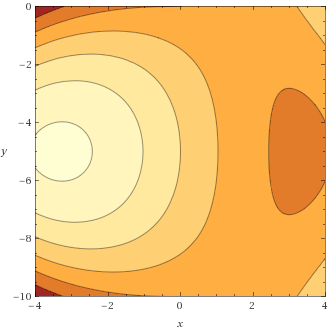
\includegraphics[width=0.8\textwidth]{../tex-snippets/ex-fn-extrema-6-img-c.png}
  \caption{Konturplot von $f(x,y) = 4(x-2)(y^2+10y)+3x^3$. Man erkennt die beiden Extremstellen. (dunkel: niedrige Funktionswerte, hell: große Frunktionswerte)}
  \label{ex-fn-extrema-6-img-c}
\end{figure}

\begin{figure}[ht]
  \centering
  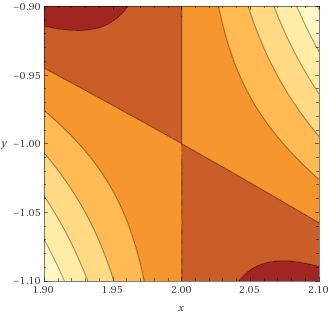
\includegraphics[width=0.8\textwidth]{../tex-snippets/ex-fn-extrema-6-img-d.png}
  \caption{Konturplot von $f(x,y) = 4(x-2)(y^2+10y)+3x^3$. Man erkennt eine Sattelstelle. (dunkel: niedrige Funktionswerte, hell: große Frunktionswerte)}
  \label{ex-fn-extrema-6-img-d}
\end{figure}

\begin{figure}[ht]
  \centering
  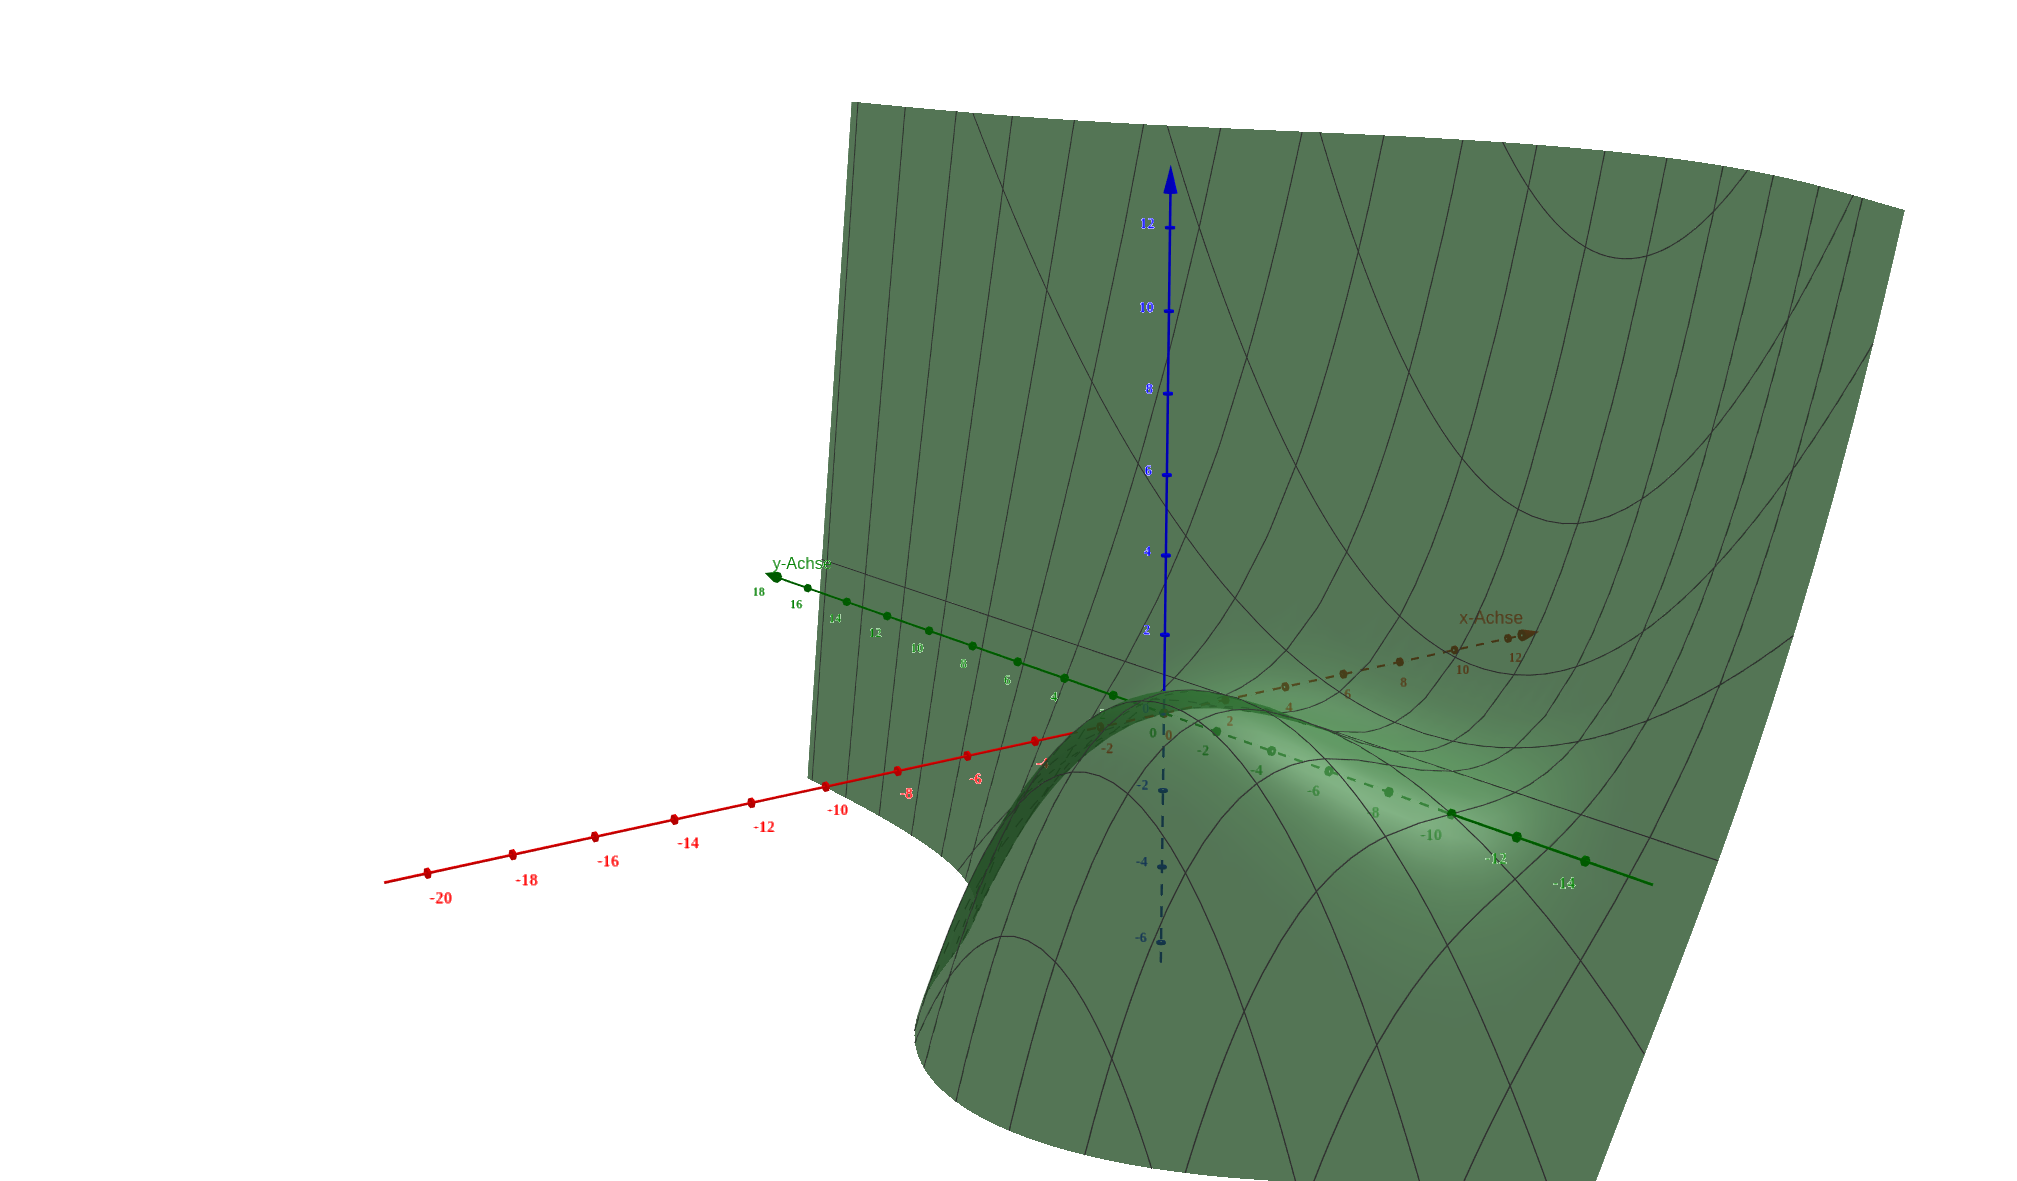
\includegraphics[width=0.8\textwidth]{../tex-snippets/ex-fn-extrema-6-img-a.png}
  \caption{3D-Plot von $f(x,y) = 4(x-2)(y^2+10y)+3x^3$}
  \label{ex-fn-extrema-6-img-a}
\end{figure}

\begin{figure}[ht]
  \centering
  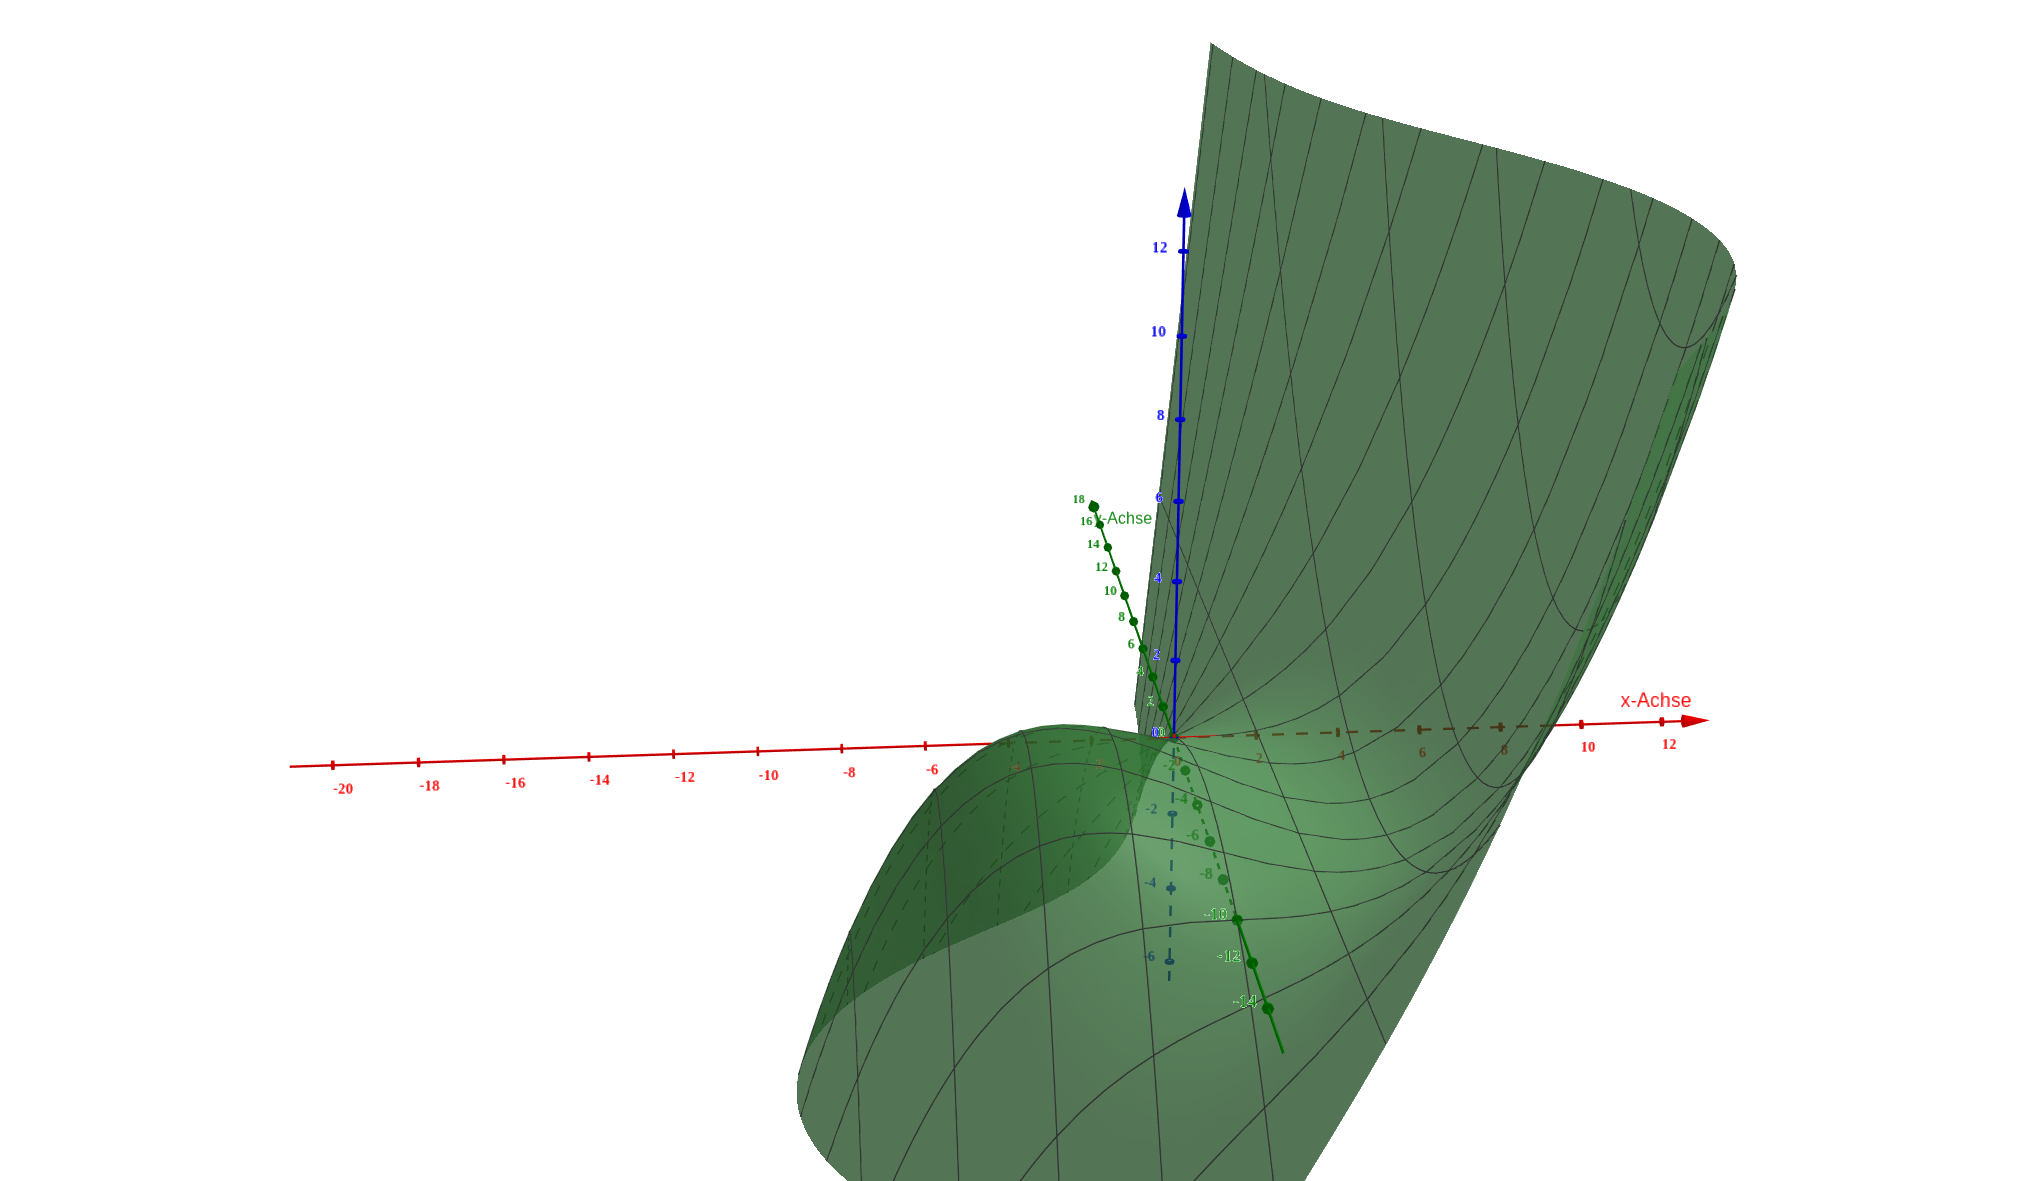
\includegraphics[width=0.8\textwidth]{../tex-snippets/ex-fn-extrema-6-img-b.png}
  \caption{3D-Plot von $f(x,y) = 4(x-2)(y^2+10y)+3x^3$}
  \label{ex-fn-extrema-6-img-b}
\end{figure}

